\chapter{Transport coefficients in the conformal window}
\label{CW}

Gauge theories with a nontrivial infrared (IR) fixed point are important in the context of model building Beyond the Standard Model \cite{Sannino:2008ha}. These theories are characterised by scale invariance in the infrared and, in the case of four space-time dimensions, they are invariant under the larger group of conformal transformations. For this reason, the region in theory space, parametrised by the number of colours ($N$) and fermion flavours ($N_f$), such that a nontrivial IR fixed point exists, is called conformal window.
Substantial effort has been taken in studying the properties of theories in the conformal window, both perturbatively  \cite{Ryttov:2010iz,Pica:2010xq,Mojaza:2012zd,Ryttov:2013hka,Ryttov:2013ura,Ryttov:2014nda,Ryttov:2016ner,Ryttov:2016asb,Ryttov:2016hal,Ryttov:2017toz,Ryttov:2017dhd,Ryttov:2017kmx} and via lattice simulations (for recent reviews see \cite{Svetitsky:2017xqk,Pica:2017gcb}). In this chapter, we present a study of the transport coefficients of theories in the perturbative conformal window, which has been published in \cite{Toniato:2016twr}. 
The chapter is organised as follows: we start by introducing the conformal window and the definition of the transport coefficients under analysis. We then describe the method used by the authors of \cite{Arnold:2000dr} for calculating the transport coefficients of a high temperature gauge theory. Finally, we present the results obtained by applying the perturbative results of \cite{Arnold:2000dr} to theories in the conformal window.  

%%%%%%%%%%%%%%%%%%%%%%%%%%%%%%%%%%%%%%%%%%%%%%%%%%%%%%

\section{The conformal window}
\label{ conformal_window}

We consider a non-Abelian gauge theory, with gauge group SU($N$) and $N_f$ fermions in the representation $r$. The two-loop beta function for the gauge coupling $g$ is given by:
 \begin{equation}
 \beta (g) = - \frac{\beta_0}{(4\pi)^2} g^3 - \frac{\beta_1}{(4\pi)^4} g^5 + \mathcal{O}(g^{7}) \; ,
 \label{beta_f}
 \end{equation}
%
with
 \begin{align}
\beta_0 &= \frac{11}{3} C_2[G] - \frac{4}{3} T[r] N_f\; , \\
\beta_1 &= \frac{34}{3} C_2^2[G] - \left ( \frac{20}{3} C_2[G] + 4 C_2[r] \right ) T[r] N_f\; ,
\end{align}
%
where $G$ denotes the adjoint representation. The definition of the group theory factors $C_2$, $T$ and $d$ can be found in appendix \ref{SUN_generators}. If $\beta_0 > 0$, the theory is asymptotically free, i.e. $g=0$ is an ultraviolet(UV)-stable fixed point of the renormalisation group (RG) flow. This happens provided the number of fermions is smaller than the upper limit:
\begin{equation}
N_f^{AF} = \frac{11}{4} \frac{C_2[G]}{T[r]} \: .
\label{NfAF}
\end{equation}
%
The number of flavours and colours can be chosen such that $\beta_0>0$ and $\beta_1<0$. In this case there exists an additional zero of the beta function:
\begin{equation}
g^* = -(4 \pi)^2 \frac{\beta_0}{\beta_1} \: .
\label{BanksZaks}
\end{equation}
%
This is an IR-stable fixed point, which can be studied in perturbation theory in case $g^*$ is small \cite{Banks:1981nn}. In particular, $g^*$ goes to zero in the limit $N_f \to N_f^{AF}$. If $g^*$ is small, the theory remains perturbative along the whole RG flow, from the UV, where it is dominated by the asymptotically free fixed point $g=0$, down to the IR. If $g^*$ is not small enough, then one has to consider higher-order terms in the beta function \ref{beta_f}, and eventually, when $g^*$ leaves the perturbative regime, apply non-perturbative methods such as lattice simulations. In theory space, parametrised by $N$ and $N_f$, the upper boundary of the conformal window for every fixed $N$ is given by $N_f = N_f^{AF}$, while the lower boundary is yet to be found via non-perturbative methods, since the value of $g^*$ increases with decreasing $N_f$.


\begin{figure}[b!]
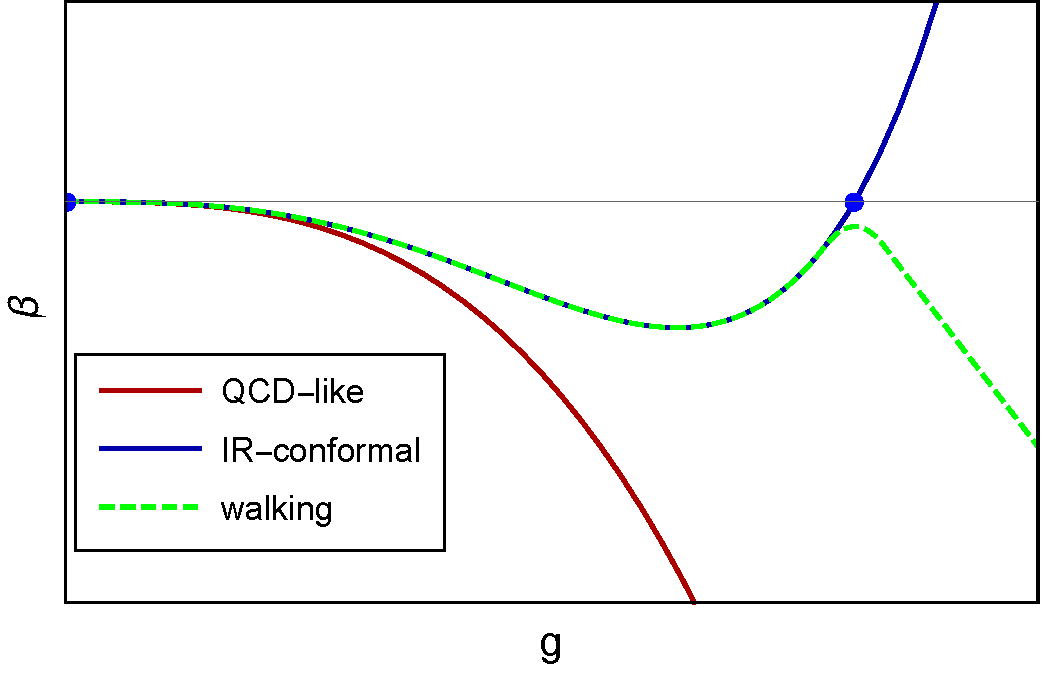
\includegraphics[width=0.5\textwidth]{pics/beta_walking}~~~
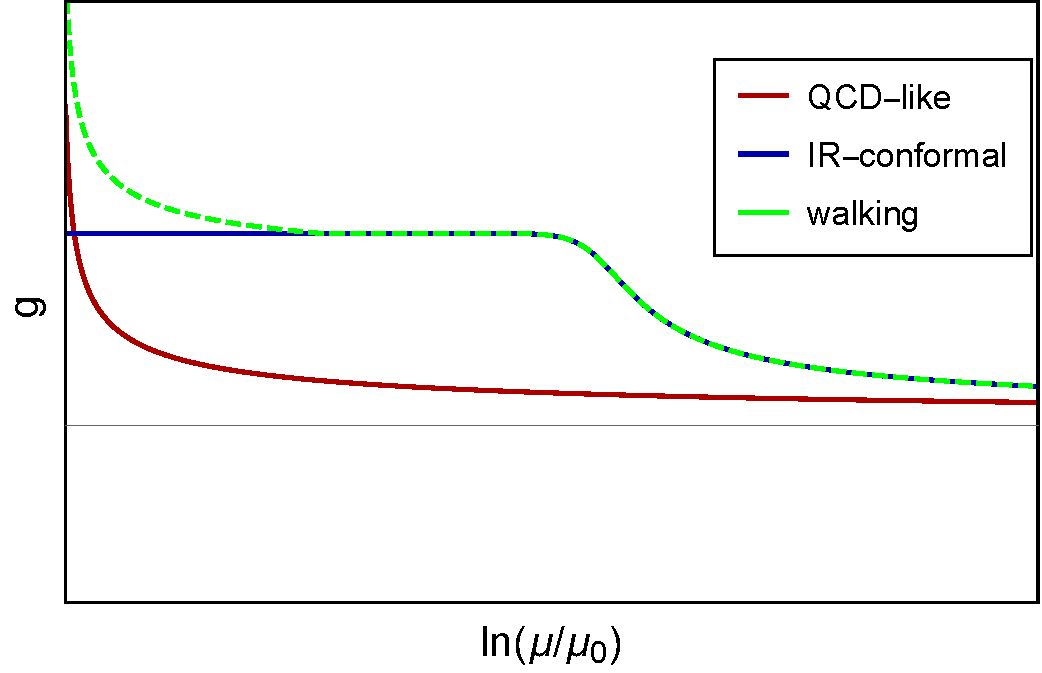
\includegraphics[width=0.5\textwidth]{pics/g_walking}
\caption{Beta function (left panel) and gauge coupling (right panel) for three different kinds of theories: a QCD-like theory (red line), a theory in the conformal window (blue line) and a theory with walking gauge coupling (green dashed line). In the right panel, the gauge coupling is plotted as a function of the energy scale $\mu$ over some reference scale $\mu_0$.} 
\label{walking}
\end{figure}


Figure \ref{walking} shows three different regimes of the beta function, and the related running of the gauge coupling. The first one (red line) characterises a QCD-like theory. The beta function has one single zero at $g=0$, and is negative for all other values of $g$. In this case, the coupling goes to zero in the UV (asymptotic freedom) and grows when moving towards the IR, until it diverges at some finite energy scale. 
This theory displays spontaneous chiral symmetry breaking in the IR. The second regime (blue line) characterises a theory in the conformal window. The beta function has two zeros, $g=0$ and $g=g^*$, and is negative in between. The gauge coupling goes to zero in the UV, and stabilises at the fixed point value $g=g^*$ in the IR. 
This theory is characterised by scale invariance in the IR, and does not display spontaneous chiral symmetry breaking. 
If the transition between the two regimes is continuous, theories with an approximate IR fixed point can be found close to the lower boundary of the conformal window. 
This third regime (green dashed line) is associated to "walking" dynamics.
The beta function is very similar to the one of theories in the conformal window, with the difference that it gets very close to zero at $g\simeq g^*$, without actually reaching a fixed point, and then assumes a QCD-like behaviour for larger values of $g$. In this theory the gauge coupling goes to zero in the UV, then stabilises at an approximately constant value for a wide range of energies, and finally diverges at a finite energy scale, thus triggering chiral symmetry breaking. 
Theories with walking gauge coupling are very important in the context of composite Higgs models, as discussed in section \ref{partial_comp}. In fact these theories show an approximate IR conformal behaviour, which can lead to a nice separation of scales and good scaling properties of composite operators, and at the same time break chiral symmetry, which is a necessary ingredient in composite Higgs models.
Lattice simulations can be used in order to find out whether a theory is in one of the three regimes shown in figure \ref{walking}, see for example \cite{Hietanen:2008mr,Hansen:2017ejh}.

Here we consider theories in the perturbative conformal window, i.e. $N_f \lesssim N_f^{AF}$, and we study their shear viscosity and fermion number diffusion coefficient by applying the perturbative results obtained in \cite{Arnold:2000dr}.

%REMEMBER TO JUSTIFY THE FACT THAT THE NUMBER OF FLAVOURS IS TREATED LIKE A CONTINUOUS PARAMETER!

%%%%%%%%%%%%%%%%%%%%%%%%%%%%%%%%%%%%%%%%%%%%%%%%%%%%%%

\section{Transport coefficients}

Transport coefficients characterise the response of a fluid to small deviations from thermodynamic equilibrium. The transport coefficients considered in our study are viscosity and diffusion coefficients. Viscosity describes the response to spacial variations of the flow velocity, in the presence of dissipative phenomena (internal friction). Diffusion coefficients describe the evolution of the density of conserved charges, when the charge concentration is not uniform over the fluid. In this section we introduce the equations of motion of a viscous fluid and the diffusion equation, which provide the definitions of the transport coefficients under analysis.

\subsection{Viscosity}

In this derivation we follow the lines of \cite{landau2013fluid}. We start by considering the motion of an ideal fluid, which is described by the continuity equation:
\begin{equation}
\partial_t \rho + \partial_i (\rho v_i) = 0 \: ,
\end{equation}
%
and Euler's equation (given here in component form):
\begin{equation}
\partial_t v_i +  v_j \partial_j v_i = -\frac{1}{\rho} \partial_i p \: ,
\end{equation}
%
where time is denoted by $t$, spacial coordinates by $x_i$ ($i=1,2,3$), the fluid mass density by $\rho$, the flow velocity components by $v_i$,  and the pressure by $p$. Sums over repeated indices are understood. Euler's equation can be rewritten as:
\begin{equation}
\partial_t (\rho v_i) = - \partial_j \Pi_{ij} \: ,
\label{Euler}
\end{equation}
%
where the symmetric tensor $\Pi_{ij} = p \delta_{ij} + \rho v_i v_j$ represents the flux density of the momentum component $i$ in all possible directions $j$. The momentum transfer described by $\Pi_{ij}$ is reversible, and it is due to the mechanical transport of volumes of fluid and to pressure forces acting in the fluid. The motion of a viscous fluid is characterised by an extra, irreversible, transfer of momentum, occurring from points where the flow velocity is large to points where it is low.
In the case of a viscous fluid, the tensor $\Pi_{ij}$ can be parametrised as:
\begin{equation}
\Pi_{ij} = p \delta_{ij} + \rho v_i v_j - \sigma_{ik} \: ,
\end{equation}
%
where $-\sigma_{ik}$ is the contribution due to internal friction. Always following \cite{landau2013fluid}, we notice that $\sigma_{ik}$ must depend on the spacial derivatives of the flow velocity, since internal friction occurs only when different layers of fluid move with respect to each other, and must vanish when the flow velocity is constant in space. Moreover, $\sigma_{ij}$
must vanish when the fluid is in uniform rotational motion, because in this case there is no relative motion between different layers of fluid. The flow velocity of a uniformly rotating fluid is expressed as: $\vec v = \vec \Omega \times \vec r$, $\vec r$ being the distance from the centre of rotation and $\vec \Omega$ the constant angular velocity. If the velocity gradients are small, we may assume that $\sigma_{ik}$ is a linear function of the first derivatives of the flow velocity. The most general function of this sort, which vanishes in case $\vec v = \mathrm{constant}$, or $\vec v = \vec \Omega \times \vec r$, is:
\begin{equation} 
\sigma_{ij} = \eta \biggl( \partial_i v_j + \partial_j v_i -\frac{2}{3} \delta_{ij} \partial_k v_k \biggr) + \zeta \delta_{ij} \partial_{k} v_k \: ,
\label{viscosity_classical}
\end{equation}
%
where the coefficient $\eta$ is the shear viscosity and $\zeta$ the bulk viscosity. The terms in equation \ref{viscosity_classical} are organised so that the expression in parentheses vanishes when traced over $i$ and $j$. To conclude, for a viscous fluid
\begin{equation}
\Pi_{ij} = p \delta_{ij} + \rho v_i v_j - \eta \biggl( \partial_i v_j + \partial_j v_i -\frac{2}{3} \delta_{ij} \partial_k v_k \biggr) - \zeta \delta_{ij} \partial_{k} v_k \: ,
\label{Navier-Stokes}
\end{equation}
%
and Euler's equation is substituted by the Navier-Stokes equation, obtained by inserting \ref{Navier-Stokes} in \ref{Euler}.


Relativistic fluid equations describe a fluid whose flow velocity is relativistic, or whose microscopical components move at relativistic speed. In order to derive them, we introduce the energy-momentum tensor $T^{\mu\nu}$ of the relativistic fluid. The component $T^{00}$ is the fluid energy density, $T^{i0} = T^{0i}$ is the momentum component density (equal to the energy flux density), and $T^{ij}$ the momentum flux density, analogue to the non-relativistic $\Pi_{ij}$. The equations of motion
\begin{equation}
\partial_{\mu} T^{\mu\nu} = 0
\end{equation}
%
express the conservation of energy and momentum in the fluid.
We start by defining $T^{\mu\nu}$ for an ideal fluid in the local rest frame. In the local rest frame, the momentum density is zero ($T^{0i} = 0$), and the force exerted by the fluid on some surface is the same in all directions, and always perpendicular to the surface. The $i$-th component of the force exerted on an infinitesimal surface $\mathrm{d} \hat \Sigma = \abs{\mathrm{d}\Sigma} \: \hat n$ is given by:  $T^{ij} \mathrm{d} \hat \Sigma^j $, where $\hat n$ is the normal to the surface. It follows from the above argument that $T^{ij} \mathrm{d} \hat \Sigma^j = p \: \mathrm{d} \hat \Sigma^i $, and therefore $T^{ij} = \delta^{ij} p$. Consequently, in the local rest frame:
 \begin{equation}
 (T^{\mu\nu}) =
 \begin{pmatrix}
 e & 0 & 0 & 0 \\
 0 & p & 0 & 0 \\
 0 & 0 & p & 0 \\
 0 & 0 & 0 & p \\
 \end{pmatrix} \: ,
 \label{T_rest_frame}
 \end{equation}
 %
 where $e$ is the energy density and $p$ the pressure.
 This expression can be generalised to a generic reference frame by introducing the fluid four-velocity $u^{\mu}$, given by $u^0 =1$, $u^i =0$ in the local rest frame, and by $u^0 = 1/\sqrt{1-v^2}$, $u^i = v^i/\sqrt{1-v^2}$ in a frame in which the fluid element moves with velocity $\vec v$. In a generic frame, $T^{\mu\nu}$ is expressed as:
  \begin{equation}
 T^{\mu\nu} = (e+p) u^{\mu} u^{\nu} - p \: \eta^{\mu\nu} \: ,
 \label{Tmunu}
 \end{equation}
 %
 where $\eta_{\mu\nu}$ is Minkowski metric. Equation \ref{T_rest_frame} is recovered by fixing $u^0 =1$, $u^i =0$.
In the presence of internal friction, further terms must be added to the energy momentum tensor \ref{Tmunu}. In the local rest frame, the spatial components of the energy momentum tensor of a viscous relativistic fluid are given by:
\begin{equation}
T_{ij} = p \delta_{ij} - \eta \biggl( \partial_i u_j +\partial_j u_i - \frac{2}{3} \delta_{ij} \partial_k u_k \biggr) - \zeta \delta_{ij} \partial_k u_k \: ,
\label{viscosity_def}
\end{equation}
%
which reduce to \ref{Navier-Stokes} in the non-relativistic limit $\abs{\vec v} \ll 1$. Equation \ref{viscosity_def} may be regarded as the definition of the shear and bulk viscosities of a relativistic fluid.
 
 \subsection{Diffusion coefficient}
 
We have seen that the equations of motion of a relativistic fluid express the conservation of energy and momentum. Further conservation laws, of the form
  \begin{equation}
 \partial_{\mu} j^{\mu} = 0 \: ,
 \label{cons_density}
 \end{equation}
 %
 exist for all other eventual conserved quantities. We consider here the case of a conserved particle number density. The current $j^{\mu}$ in this case is expressed as: $j^{\mu} = n  u^{\mu}$, where $u^{\mu}$ represents the fluid four-velocity and $n$ the particle number density in the local rest frame. The diffusion equation:
  \begin{equation}
 \partial_t n = D \Laplace n \: ,
 \label{diffusion_eq}
 \end{equation}
 %
 where $\Laplace = \partial_i \partial^i$, describes the evolution of the number density $n$, when $n$ is low and not uniform over the fluid. In this case, the number density flux can be expressed, in the local rest frame, as:
 \begin{equation}
j^i = - D \partial^i n \: ,
\label{diffusion_current}
\end{equation}
%
which, in combination with the conservation law \ref{cons_density}, implies the diffusion equation \ref{diffusion_eq}. The coefficient $D$ is known as diffusion coefficient. Equations of the form \ref{diffusion_eq}, \ref{diffusion_current} describe for example the evolution of the concentration $c$ of the solute in a weak solution ($c \ll 1$) \cite{landau2013fluid}. Random walk dynamics, which may be applied to the description of Brownian motion, is also governed by the diffusion equation. It will be shown in the following that the current related to fermion number conservation (analogue to baryon number conservation in QCD) in a hot gauge theory satisfies a constitutive relation of the form \ref{diffusion_current}. 

%In particular, in a SU($N$) gauge theory, if the temperature is high enough, the whole set of currents related to SU($N_f$)$_L \times$SU($N_f$)$_R \times$ U(1)$_B \times$ U(1)$_A$ flavour symmetry, is conserved. This is a good approximation when 


%%%%%%%%%%%%%%%%%%%%%%%%%%%%%%%%%%%%%%%%%%%%%%%%%%%%%%

\section{Transport coefficients of a hot gauge theory: kinetic approach}

The equilibrium state of a high temperature quantum field theory can be described as a relativistic fluid. Transport coefficients can in principle be computed, based on the dynamics of the underlying microscopic theory.
This is what the authors of \cite{Arnold:2000dr,Arnold:2003zc} did in the case of a weakly coupled , high temperature gauge theory, both in a leading-log approximation \cite{Arnold:2000dr} and in a full leading order treatment \cite{Arnold:2003zc}.
In this section, we describe the method used in these works to compute the transport coefficients. The analytic results given in \cite{Arnold:2000dr}, together with the coefficients in table \ref{AB}, are the basis for our study of transport coefficients in the perturbative conformal window.

In \cite{Arnold:2000dr,Arnold:2003zc}, a finite temperature gauge theory coupled to fermions is considered, under the assumption that the gauge coupling at the scale of the temperature is weak: $g(T) \ll 1$. The temperature is assumed to be much larger than any other mass scale in the theory, such as for example zero-temperature fermion masses, chemical potentials, or, in the case of non-Abelian gauge group, the scale at which the gauge coupling becomes strong. Under this assumption, the transport coefficients are given by a power of the temperature determined by dimensional analysis, multiplied by some function of the gauge coupling.

As explained by the authors of \cite{Arnold:2000dr,Arnold:2003zc}, a kinetic theory approach is appropriate for computing the transport coefficients under their analysis (shear viscosity, diffusion coefficients, electrical conductivity) at leading order in the gauge coupling. We will get back to this point in the following. The kinetic theory is defined by assigning to each particle species a phase space distribution function $f^a(\vec p, x)$, which satisfies a Boltzmann equation of the form:
\begin{equation}
\biggl( \pder{ }{t}+ \vec v_{\vec p} \cdot \pder{ }{\vec x} + \vec F \cdot \pder{ }{\vec p} \biggr) f^a(\vec p,x) = -C_a[f] (\vec p,x) \: ,
\end{equation}
%
where $\vec v_{\vec p}$ is the velocity of a particle with momentum $\vec p$, $\vec F$ is an external force acting on the particle species $a$, and $C_a[f](\vec p, x)$ is the collision term, describing the rate at which excitations with momentum $\vec p$ of the species $a$ are lost or created due to scattering with other particles in the fluid. Typical excitations in the plasma have momentum $\abs{\vec p} = \mathcal O(T)$ and thus are highly relativistic (in the high temperature limit), and may be treated as massless particles moving at the speed of light, with dispersion relation $p^0= \abs{\vec p}$. It follows that the velocity $\vec v_{\vec p}$ is a unit vector: $\vec v_{\vec p} = \hat p = \vec p/ \abs{\vec p}$. 

In \cite{Arnold:2000dr} transport coefficients are computed in the leading-log approximation, i.e. the coefficient of the leading order result (in the gauge coupling $g$) is in turn expanded in powers of $1/\log{g^{-1}}$ and only the first term of this expansion is retained. In this approximation, it is sufficient to include in the collision term only two-body scattering processes:
\begin{equation}
\begin{split}
C_a[f](\vec p, x)  & = \frac{1}{4 p^0} \sum_{b,c,d}^{\mathrm{f \bar f h c}} \int_{\vec k, \vec{p'}, \vec k'} \abs{\mathcal M^{ab}_{cd}(p,k;p',k')}^2 (2 \pi)^4 \delta^4(p+k-p'-k') \times \\
& 
\begin{split}
\times  \biggl[ & f^a(\vec p,x) f^b(\vec k,x) [1 \pm f^c(\vec{p'},x)] [1 \pm f^d(\vec k',x)] - \\ 
& - f^c(\vec{p'},x) f^d(\vec k',x)[1 \pm f^a(\vec p,x)] [1 \pm f^b(\vec k,x)] \biggr]  \: ,
\end{split}
\end{split}
\end{equation}
%
where $\mathcal{M}^{ab}_{cd}$ is the scattering amplitude for the process $ab \leftrightarrow cd$, and the sum extends to flavours (f), anti-flavours ($\mathrm{\bar f}$), helicities (h) and colours (c) of the particles $b$, $c$ and $d$. The shorthand notation $\int_{\vec p} \equiv \int \mathrm{d}^3p/\bigl(2p^0 (2 \pi)^3\bigr)$ is introduced for the momentum integrals, and in the final-state statistical factors $[1 \pm f]$ the upper sign applies to bosons and the lower to fermions. 
The energy momentum tensor of the fluid formed by the excitations distributed according to $f^a$ is given by:
\begin{equation}
T^{\mu\nu}(x) = \sum_a^{\mathrm{f \bar f h c}} \int \frac{\mathrm d^3 p}{(2 \pi)^3 p^0} p^{\mu} p^{\nu} f^a(\vec p, x) \: ,
\label{Tmunu_kinetic}
\end{equation}
%
while other conserved currents are given by:
\begin{equation}
j^{\mu}(x) = \sum_a^{\mathrm{f \bar f h c}}\int \frac{\mathrm d^3 p}{(2 \pi)^3 p^0} p^{\mu} q^a f^a(\vec p, x) \: ,
\label{jmu_kinetic}
\end{equation}
%
where $q^a$ is the corresponding charge carried by the species $a$.



The next step in the computation of transport coefficients is the linearisation of the Boltzmann equation in the case of small deviations from local equilibrium. Equilibrium solutions of the Boltzmann equation are given by:
\begin{equation}
f^a_{eq}(\vec p) = \frac{1}{\exp[\beta(- u_{\mu}p^{\mu} - \mu_{\alpha}q_{\alpha}^a)] \mp 1} \: ,
\label{equilibrium}
\end{equation}
%
where $\beta = 1/T$, $u^{\mu}$ is the fluid four-velocity, $\set{q^a_{\alpha}}$ a set of conserved charges and $\set{\mu_{\alpha}}$ the related chemical potentials. As before, the upper sign applies to bosons and the lower to fermions, and this convention will hold through all the following derivation. In order to study small deviations from local equilibrium, relevant for the computation of transport coefficients, the phase space distribution can be written as:
\begin{equation}
f^a(\vec p, x) = f_0^a(\vec p, x) + \delta f^a (\vec p, x) \: ,
\end{equation}
%
where $f_0^a(\vec p, x)$ is a local equilibrium solution, i.e. of the form \ref{equilibrium} but with $\beta$, $u_{\mu}$, $\mu_{\alpha}$ possibly depending on space-time coordinates. The deviation from local equilibrium $\delta f^a$ can be rewritten in a form that will simplify the expression of the linearised collision term:
\begin{equation}
 \delta f^a (\vec p, x)= f_0^a(\vec p, x) [1 \pm f_0^a(\vec p, x)] f_1^a(\vec p, x) \: .
\end{equation}
%
The Boltzmann equation can be linearised by retaining only terms of first order in the deviation from equilibrium. In particular, only terms that are linear in either $f^a_1$, the external force $\vec F$ or the gradients of $\beta$, $u_{\mu}$, $\mu_{\alpha}$ are retained. Products of $f^a_1$ with gradients or $\vec F$, as well as derivatives of $f^a_1$, are among the discarded terms. As a result, the Boltzmann equation becomes a linear integral equation in $f^a_1$:
\begin{equation}
\biggl( \pder{ }{t}+ \hat p \cdot \pder{ }{\vec x} + \vec F \cdot \pder{ }{\vec p} \biggr) f^a_0(\vec p,x)  =
- (\mathcal Cf_1)^a (\vec p, x) \: ,
\label{lin_boltzmann}
\end{equation}
%
where the linearised collision integral is given by:
\begin{equation}
\begin{split}
(\mathcal Cf_1)^a (\vec p, x) =  \frac{1}{4 p^0} \sum_{b,c,d}^{\mathrm{f \bar f h c}} &\int_{\vec k, \vec{p'}, \vec k'}  \abs{\mathcal M^{ab}_{cd}(p,k;p',k')}^2 (2 \pi)^4 \delta^4(p+k-p'-k') \times \\
&\times f_0^a(\vec p,x) f_0^b(\vec k,x)[1 \pm f_0^c(\vec{p'},x)][1 \pm f_0^d(\vec k', x)] \times \\
& \times \bigl[f_1^a(\vec p,x) + f_1^b(\vec k,x) - f_1^c(\vec{p'},x) - f_1^d(\vec k',x)\bigr] \: .
\end{split}
\label{lin_coll_integral}
\end{equation}
%
In order to obtain this result, the fact that the collision term vanishes in the case of a local equilibrium distribution, $C_a[f_0] = 0$, has been used.

In this setup, transport coefficients can be computed by applying the following program:
\begin{itemize}
\item the collision integrals \ref{lin_coll_integral} must be computed for all the relevant particle species, at the desired order in the gauge coupling $g$,
\item an appropriate "driving term" (left-hand-side of \ref{lin_boltzmann}) must be chosen, which allows to compute the desired transport coefficient,
\item the deviations from local equilibrium $f_1^a$ must be computed for all relevant particle species by solving the integral equations \ref{lin_boltzmann},
\item the phase space distributions $f^a = f^a_0 + \delta f^a$ must be inserted in the relevant conserved current (\ref{Tmunu_kinetic} or \ref{jmu_kinetic}). Transport coefficients can be read off from the resulting equation.
\end{itemize}
%
Here we don't aim at describing the full procedure in detail. We will just give a sketch of point two of the above program, and further on we will briefly discuss which approximations are applied in the collision integrals in order to obtain leading-log results for transport coefficients.

The form of the local equilibrium distribution $f_0$ can be chosen appropriately for the computation of a specific transport coefficient. In the case of viscosity, the temperature and chemical potentials are constant, while the flow velocity varies as a function of space. In the case of a diffusion coefficient, some chemical potential $\mu_{\alpha}$ is chosen as varying in space, while all other parameters are constant. In both cases the external force $\vec F$, which would be relevant for the calculation of electrical conductivity, can be set to zero. Derivatives of $f_0^a$ can be written as:
\begin{equation}
\mathrm d f_0^a(\vec p,x) = f_0^a(\vec p,x) [1 \pm f_0^a(\vec p,x)] \mathrm d [\beta u_{\mu}p^{\mu} + \beta q^a_{\alpha} \mu_{\alpha}] \: ,
\end{equation}
%
from which the left-hand-side of equation \ref{lin_boltzmann} can be expressed as (we limit ourselves to the forms of $f_0$ relevant for viscosity and diffusion coefficients):
\begin{equation}
 \hat p \cdot \pder{ }{\vec x} f^a_0(\vec p, x) = \beta f_0^a(\vec p,x) [1 \pm f_0^a(\vec p,x)] q^a I_{i \dots j} (\hat p) X_{i \dots j} (x) \: ,
\label{driving_term}
\end{equation}
%
where the term $ \hat p \cdot \partial /\partial \vec x \: [u_{\mu}p^{\mu} + q^a_{\alpha} \mu_{\alpha}]$ has been split in a part depending only on spacial coordinates:
\begin{equation}
X_{i \dots j} (x) =
\begin{cases}
\pder{ }{x^i} \mu_{\alpha} & \mbox{(diffusion coefficient)} \\
\frac{1}{\sqrt 6} \bigl( \pder{ }{x^i} u_j + \pder{ }{x^j} u_i -\frac{2}{3} \delta_{ij} \pder{ }{x^k} u_k \bigr) & \mbox{(shear viscosity)}
\end{cases}
\end{equation}
%
and one depending only on the direction of the momentum $\hat p$:
\begin{equation}
I_{i \dots j} (\hat p)=
\begin{cases}
\hat p_i & \mbox{(diffusion coefficient)} \\
\sqrt{\frac{3}{2}} \bigl(\hat p_i \hat p_j - \frac{1}{3}\delta_{ij} \bigr) & \mbox{(shear viscosity)} \: .
\end{cases}
\end{equation}
%
In equation \ref{driving_term}, $q^a$ is the relevant conserved charge, and it stands for either $q^a_{\alpha}$ (for the diffusion coefficient) or $\abs{\vec p}$ (for shear viscosity).

 We now assume to be in the local rest frame of the fluid. In this frame, at any point $x$, $f_0(\vec p,x)$ depends only on $p^0 = \abs{\vec p}$, and all the angular dependence in \ref{driving_term} comes from the function $I_{i \dots j}(\hat p)$. The linearised collision operator $\mathcal{C}$, in the local rest frame at $x$, is rotationally invariant and independent of $x$, therefore the dependence of $f_1^a$ on $\hat p$ and $x$ is the same as the one of the driving term \ref{driving_term}. As a consequence, the deviation from local equilibrium $f_1^a$ can be expressed as:
  \begin{equation}
 f_1^a (\vec p,x) = \beta^2 X_{i \dots j} (x) I_{i \dots j} (\hat p) \chi^a(\abs{\vec p}) \: ,
 \label{f1}
 \end{equation}
 %
 where $\chi^a(\abs{\vec p})$ is an unknown function, which must be determined by solving the integral equation \ref{lin_boltzmann}. The phase space distributions $f^a(\vec p,x)$ thus obtained should then be used to compute the energy momentum tensor \ref{Tmunu_kinetic}  and the conserved current \ref{jmu_kinetic}. In the case of the energy momentum tensor, the forms of $X_{i \dots j}(x)$ and $I_{i \dots j}(\hat p)$ relevant for the computation of shear viscosity must be chosen. It can be seen that the deviation from local equilibrium $\delta f$ contributes to $T^{\mu\nu}$ with a term of the form
  \begin{equation}
 \eta \biggl( \pder{ u_j}{x^i}  + \pder{ u_i}{x^j}  -\frac{2}{3} \delta_{ij} \pder{ u_k}{x^k}  \biggr) \: ,
 \end{equation} 
 %
where the coefficient $\eta$, representing the shear viscosity, can be computed once the functions $\chi^a(\abs{\vec p})$ are known for all relevant particle species. In the case of the diffusion coefficient, it can be seen that the current \ref{jmu_kinetic} is of the form \ref{diffusion_current}, once the term $\partial \mu_{\alpha}/\partial x^i$ is rewritten as:
\begin{equation}
\pder{\mu_{\alpha} }{x^i}  = \biggl(\pder{n_{\alpha}}{ \mu_{\alpha}}\biggr)^{-1} \pder{n_{\alpha} }{x^i}  \: .
\end{equation}
%
In fact, in the local rest frame, only the deviation from local equilibrium $\delta f$ gives a nonzero contribution to the spacial components $j^i$.
The diffusion coefficient $D_{\alpha}$, relative to the conserved charge $q_{\alpha}$, can be computed once the functions $\chi^a(\abs{\vec p})$ are determined by solving the linearised Boltzmann equation \ref{lin_boltzmann} in the presence of the appropriate driving term.

The kinetic theory approach is not appropriate for describing all the excitations of a high temperature gauge theory. The authors of \cite{Arnold:2000dr,Arnold:2003zc} argue that soft excitations with momentum $\mathcal O(gT)$ or less cannot be described in terms of quasiparticles with purely local collisions. These long-wavelength fluctuations must be treated as classical gauge field fluctuations, and an effective theory can be constructed in which the high-momentum excitations propagate in a slowly varying classical background field. The method described above for the computation of transport coefficients is valid only for those quantities that are not dominantly sensitive to soft excitations. This is true for shear viscosity and diffusion coefficients, but not for bulk viscosity, which would require a more refined treatment \cite{Arnold:2000dr}.

 
\subsection{Leading-log and next-to-leading-log results}

In \cite{Arnold:2000dr}, leading-log results are provided for shear viscosity, fermion number diffusion coefficient and electrical conductivity. The leading-log approximation is obtained by restricting to a specific interval the integration over the transfer momentum in the collision integral \ref{lin_coll_integral}. In a process with ingoing momenta $\vec p$, $\vec k$ and outgoing momenta $\vec{p'}$, $\vec k'$, the transfer momentum can be defined as $\vec q = \vec{p'} - \vec p$. The leading-log approximation amounts to extracting the small $\abs{\vec q}$ contribution to the collision integral ($\abs{\vec q} \ll T$). In this approximation, the integration over $q \equiv \abs{\vec q}$ results in a factor:
\begin{equation}
\int_{gT}^T \frac{\mathrm d q}{q} = \log g^{-1} \: .
\end{equation}
%
The lower bound at $q = gT$ is due to the fact that some of the tree-level diagrams, which contribute at leading order in $g$ to the collision integral, are divergent at small $q$. As a consequence, the collision integral is logarithmically divergent. The infrared divergences disappear when self-energy contributions are included in the exchange lines in the diagrams. The approach assumed in \cite{Arnold:2000dr} is not to include the self-energy contributions, and to cut down the integration at $q \sim gT$, where the self-energy corrections to the propagators start becoming important. This way leading-log results are obtained.

 We report here the results for shear viscosity and fermion number diffusion coefficient, which are relevant for our study in the conformal window. The leading-log shear viscosity reads \cite{Arnold:2000dr}:
 \begin{equation}   
\eta \simeq 270 \, d [G] \zeta(5)^2 \biggl( \frac{2}{\pi} \biggr)^5 (v^T c^{-1} v) \frac{T^3}{g^4 \log( g^{-1})}\;,
\label{eta}
\end{equation}
%
where  
\begin{equation}
\begin{split}
c =  (d [G] C_2 [G]  & + N_f d [r] C_2 [r])
\begin{pmatrix}
d [G] C_2 [G] & 0 \\
0 & \frac{7}{4} N_f d [r] C_2 [r]
\end{pmatrix}
+  \\
& + \frac{9 \pi^2}{128} N_f d [r] C_2^2 [r] d [G]
\begin{pmatrix}
1 & -1 \\
-1 & 1
\end{pmatrix} \;,
\end{split}
\label{c_visc}
\end{equation}
\begin{equation}
v = 
\begin{pmatrix}
d [G] \\
\frac{15}{8} N_f d [r]
\end{pmatrix} \; .
\label{v_visc}
\end{equation}
%
In the previous equations, $N_f$ denotes the number of fermions, $r$ the representation of the gauge group acting on the fermion fields and $G$ the adjoint representation. The definition of the group factors $d$ and $C_2$ can be found in appendix \ref{SUN_generators}. In equation \ref{eta}, the $\simeq$ sign is due to the fact that this is an approximate result. Specifically,  the results of \cite{Arnold:2000dr,Arnold:2003zc} are obtained by converting the solution of the integral equation \ref{lin_boltzmann} in a variational problem, corresponding to the maximisation of a functional of $\chi^a(\abs{\vec p})$ (see equation \ref{f1}). The maximisation is performed by expanding $\chi^a(\abs{\vec p})$ over a finite basis of functions, and maximising within this variational subspace. The analytic expression \ref{eta} is found by cutting to one the number of elements in the functional basis, and it approximately reproduces results obtained numerically by using a larger basis \cite{Arnold:2000dr}.


The diffusion coefficient for the net number density of the fermion flavour $a$ reads, at the leading-log level \cite{Arnold:2000dr}:
\begin{equation}
D_a \simeq \frac{6^5 \zeta(3)^2}{\pi^3 C_2[r_a]} \biggl[ \sum_b^{f \bar{f} h} T[r_b] \lambda_b + \frac{3 \pi^2}{8} 
C_2[r_a] \biggr]^{-1}  \frac{T^{-1}}{g^4 \log(g^{-1})}\;, 
\label{diff_coeff}
\end{equation}
%
where the sum extends over all flavours (f), anti-flavours ($\bar{\mathrm f}$) and helicities (h) of particles of species $b$ that $a$ can scatter with in the process $ab \to ab$ mediated by a gauge boson. Specifically, a factor of four appears for every Dirac fermion, and a factor of two for every gauge boson. The factor $\lambda_b$  is  equal to one if the particle $b$ is a fermion, and to two if it is a boson. The definition of the group factors $T$ and $C_2$ can be found in appendix \ref{SUN_generators}. This result is again obtained by using a one-function basis for the expansion of $\chi^a(\abs{\vec p})$. In the case of an SU($N$) gauge theory with $N_f$ Dirac fermions, all in the same representation $r$, the diffusion coefficient is equal for all fermion species, and it reads:
\begin{equation}
D \simeq \frac{6^5 \zeta(3)^2}{\pi^3 C_2[r]} \biggl[ 4 N_f T[r] + 4 N + \frac{3 \pi^2}{8} C_2[r] \biggr]^{-1} 
 \frac{T^{-1}}{g^4\log(g^{-1})} \;.
\end{equation}

In \cite{Arnold:2003zc}, a full leading-order computation of transport coefficients is performed, and the convergence of the expansion in inverse powers of $\log g^{-1}$ is analysed. The authors show that the leading-order transport coefficients can in turn be expanded according to:
\begin{equation}
D \sim \frac{1}{g^4 T} \sum_{n=1}^{\infty} D_n(\mu) \biggl( \log\frac{\mu}{m_D}\biggr)^{-n} \: ,
\label{D_series}
\end{equation}
\begin{equation}
\eta \sim \frac{T^3}{g^4} \sum_{n=1}^{\infty} \eta_n(\mu) \biggl( \log\frac{\mu}{m_D}\biggr)^{-n} \: ,
\label{eta_series}
\end{equation}
%
where $\mu$ is an arbitrary energy scale, which should be chosen to be $\mathcal O(T)$, and $m_D$ is the Debye mass:
 \begin{equation}
 m_D^2 =  \frac{1}{3} \left(C_2[G] + N_f C_2[r]\frac{d[r]}{d[G]}  \right)g^2 T^2 \; .
\label{Debye_mass} 
\end{equation}
%
The coefficients $\eta_1$ and $D_1$ are independent of $\mu$. The leading-log approximation corresponds to truncating the series \ref{D_series}, \ref{eta_series} at $n=1$.

The scale $\mu$ can be chosen such that the $n=2$ term in the expansion vanishes: $D_2(\mu^*) = 0$, $\eta_2(\mu^*) =0$. With this choice, the next-to-leading-log transport coefficients are given by:
\begin{equation}
D_{NLL} = \frac{1}{g^4 T} \biggl( \frac{D_1}{ \log(\mu^*/m_D)} \biggr) \: , \qquad
\eta_{NLL} = \frac{T^3}{g^4} \biggl( \frac{\eta_1}{ \log(\mu^*/m_D)} \biggr) \: .
\end{equation} 
%
We rename $\mu^* = AT$ in the case of shear viscosity, and $\mu^* = BT$ for the diffusion coefficient, and we find the next-to-leading-log results:
 \begin{equation}   
\eta \simeq 270 \, d [G] \zeta(5)^2 \biggl( \frac{2}{\pi} \biggr)^5 (v^T c^{-1} v) \frac{T^3}{g^4 \log( AT/m_D)} \; ,
\label{eta_NLL}
\end{equation}
\begin{equation}
D \simeq \frac{6^5 \zeta(3)^2}{\pi^3 C_2[r]} \biggl[ 4 N_f T[r] + 4 N + \frac{3 \pi^2}{8} C_2[r] \biggr]^{-1} 
 \frac{T^{-1}}{g^4\log(BT/m_D)} \; ,
 \label{D_NLL}
\end{equation}
%
where the matrix $c$ and the vector $v$ are always given by equations \ref{c_visc}, \ref{v_visc}. The coefficients $A$ and $B$, for an SU(3) gauge group and different values of $N_f$ in the perturbative conformal window (plus $N_f = 6$), have kindly been provided to us by G. D. Moore. Their values are reported in table \ref{AB}.

The convergence of the inverse-log expansion is studied in \cite{Arnold:2003zc}: the coefficients $D_n(\mu^*)$, $\eta_n(\mu^*)$ are found to decrease with increasing $n$ until $n=4$, while subsequent coefficients appear to grow. The authors prove that the expansions \ref{D_series}, \ref{eta_series} are asymptotic expansions with zero radius of convergence. By comparing full-leading-order results with truncated expansions, they find that the next-to-leading-log result is very close to the full leading order provided $m_D/T \leq 1$, while going beyond the order $n=2$ in the inverse-log expansion has little practical utility.

    \begin{table}[h!]
\begin{center}
    %\begin{minipage}{3.8in}
    \begin{tabular}{c||ccc }
    $N_f$ & $ \quad A$ & $\quad B $ &   \\
    \hline \hline
    $ 6 $ & \quad 2.918 & \quad 3.064   \\
        $14$ &\quad 2.878 &\quad 3.135  \\
        $15$ & \quad 2.873 & \quad 3.172 \\
        $16$ & \quad 2.869  & \quad 3.176 \\
    $16.25$ & \quad 2.867 & \quad 3.177
    \end{tabular}
    %\end{minipage}
    \end{center}
\caption{Values of the coefficients $A$ and $B$ \cite{privcommGDM}
appearing in the next-to-leading-log expressions of the shear viscosity and the fermion number diffusion coefficient, 
for $N = 3$ and different values of $N_f$.}
\label{AB}
    \end{table}


%%%%%%%%%%%%%%%%%%%%%%%%%%%%%%%%%%%%%%%%%%%%%%%%%%%%%%

\section{Application to theories in the conformal window}

We consider SU($N$) gauge theories in the perturbative conformal window, i.e. with a number $N_f$ of fermion flavours such that: $N_f \lesssim N_f^{AF}$ (see equation \ref{NfAF}). For these theories, we study the shear viscosity and fermion number diffusion coefficient, as defined in equations \ref{eta_NLL}, \ref{D_NLL}. More specifically, we concentrate on the dimensionless quantities $\eta/s$ and $DT$, $s$ being the entropy density, i.e. we drop the overall temperature dependence, which, in a hot gauge theory, is simply determined by dimensional analysis. We consider the IR-fixed-point values of $\eta/s$ and $DT$, and we study their dependence on the number of flavours for a fixed value of $N$. Moreover, we study the temperature dependence of $\eta/s$ and $DT$, due to the running of the gauge coupling, for different choices of $N$ and $N_f$ within the perturbative conformal window. 

We start by considering the dimensionless ratio $\eta/s$. We determine the entropy density $s$ via its relation with the free energy density $f$: 
\begin{equation}
s = - \der{f}{T}  \; . 
\end{equation}
%
The free energy density of a high temperature SU($N$) gauge theory with $N_f$ fermion flavours is known up to the order $g^6 \log(1/g)$ \cite{Kajantie:2002wa}, but for our study it is sufficient to retain only terms up to order $g^2$:
\begin{equation}
\frac{f}{\pi^2 T^4 } = - \frac{d[G]}{9} \left[ \frac{1}{5} + \frac{7}{20}\frac{d[r]}{d[G]}N_f 
-   \left ( C_2[G] + \frac{5}{2}T[r] N_f \right ) \frac{g^2}{(4\pi)^2} \right ]\; ,
\end{equation}
%
where $r$ is the representation of the gauge group acting on the fermions, $G$ the adjoint representation and the group theory factors $d$, $T$ and $C_2$ are defined appendix \ref{SUN_generators}.
The free energy of hot gauge theories in the perturbative conformal window has been studied in \cite{Mojaza:2010cm}. One of the interesting results of this work is a good estimate of the lower boundary of the conformal window, obtained by studying the order-$g^6 \log(1/g)$ free energy density evaluated at the IR fixed point.

In order to obtain the fixed-point value of an observable, the gauge coupling $g$ must be traded for its value at the fixed point: $g=g_{FP}$. The shear viscosity-to-entropy density ratio at a generic fixed point reads:
\begin{equation}
\biggl( \frac{\eta}{s} \biggr)^{FP} = \frac{{\cal A}(N_ f, N) }{g_{FP}^4 \ln[{\cal B}(N_f, N)g_{FP}^{-1}]}  \; , 
\label{etaoversFP}
\end{equation}
%
with $ {\cal A}(N_f, N) $  and $ {\cal B}(N_f, N) $ calculable definite positive and smooth functions of the number of 
colours and flavours.  At non-interacting fixed points,  such as the UV fixed point ($g_{FP} = 0$), the ratio diverges. On the  other hand, at the interacting IR fixed point $g_{FP} = g^*$ (see equation \ref{BanksZaks}) the ratio approaches a finite value controlled by a small non-vanishing $\delta = N_f^{AF} - N_f $. 
 
In the upper panel of figure \ref{etas_Nf}, we plot $\eta/s$ evaluated the the IR fixed point, $(\eta/s)^{IR}$, as function of the number of flavours, for fermions in the fundamental representation and $N = 3$. We express the coefficient $A$ of equation \ref{eta_NLL} as a continuous function of the number of fermions via a linear fit of the values given in table \ref{AB}. When decreasing the number of flavours below the asymptotically free boundary, where the shear viscosity diverges, we observe an abrupt decrease of $\eta/s$, while still remaining above the bound $\eta/s \geq 1/(4\pi)$ conjectured by AdS/CFT \cite{Kovtun:2004de}. We expect that, when further decreasing the number of flavours, the IR ratio would decrease to reach a minimum value at the lower boundary of the conformal window. Below this critical number of flavours we expect the onset of chiral symmetry breaking and the theory in the deep IR becomes a theory of non-interacting pions with again a divergent value of $\eta/s$.

In the lower panel of figure \ref{etas_Nf}, we present the temperature dependence of the shear viscosity over entropy 
density for several values of $N_f$. $\eta/s$ depends on the temperature over a reference scale $\Lambda$ via the 
gauge coupling. The reference energy scale is chosen such that the beta function reaches a minimum at $T=\Lambda$,
between the UV and IR fixed points:
\begin{equation}
g^2(\Lambda)=\frac{3}{5}(g^*)^2 \, .
\label{Lambda_visc}
\end{equation} 
%
For $N_f = 6$, where theory does not display an IR perturbative fixed point, $\Lambda$ is taken to be the scale at 
which the one-loop gauge coupling diverges. The ratio $\eta/s$ decreases with decreasing temperature. For $N_f=15$, we observe that a minimum develops at around $T = \Lambda$.  This happens  because for this value of $N_f$ there exists a temperature such that $4 \ln \left(AT/m_D \right)  = 1 $, which corresponds to a minimum for the function $g^{-4} \ln \left(AT/m_D \right)  ^{-1} $. 

\begin{figure}[b!]
\begin{center}
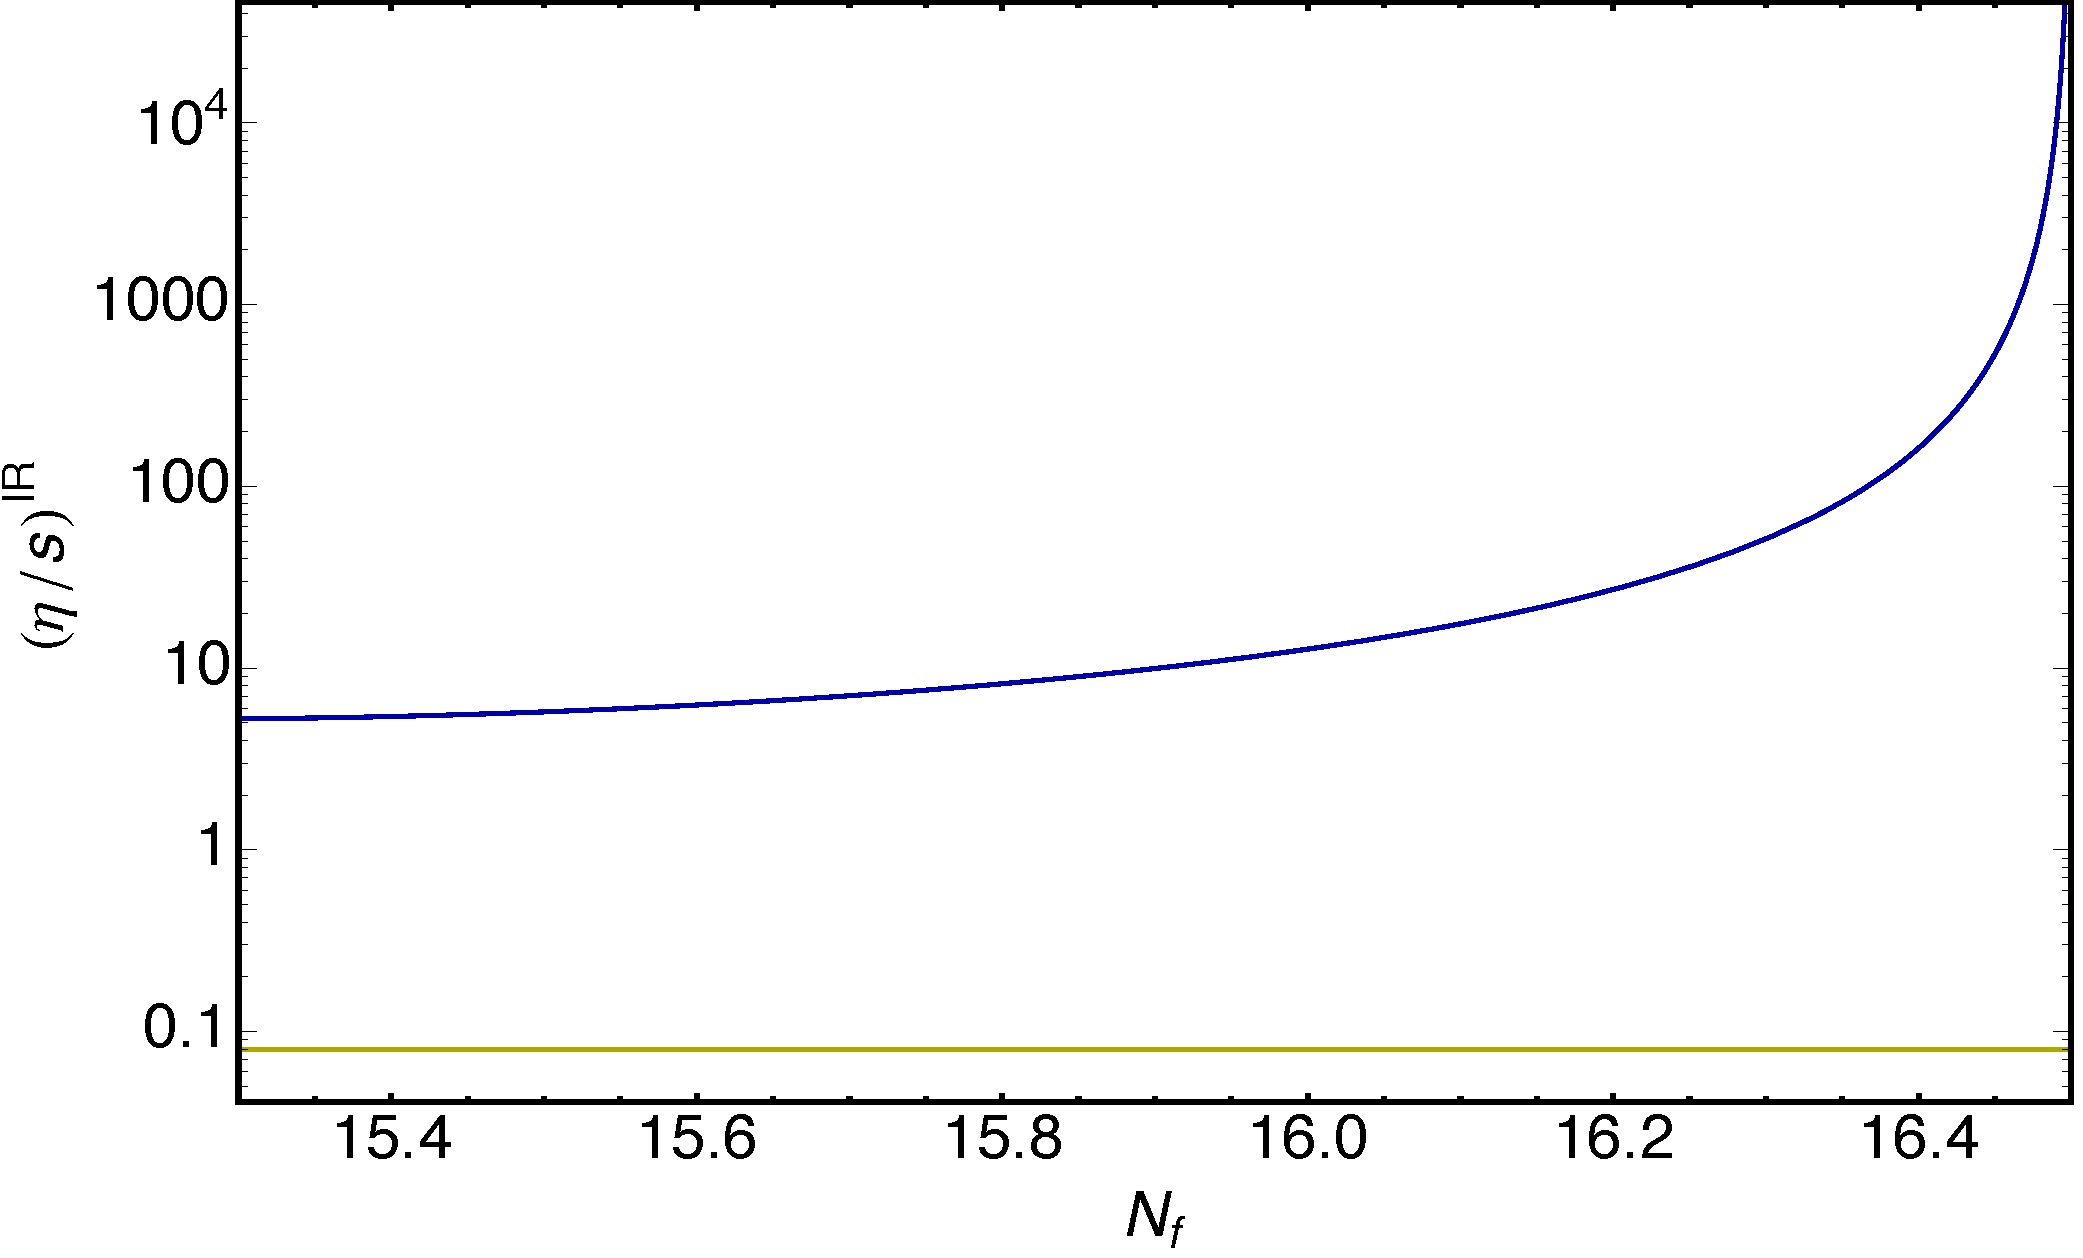
\includegraphics[width=0.665\textwidth]{pics/eta-s-n3} \\
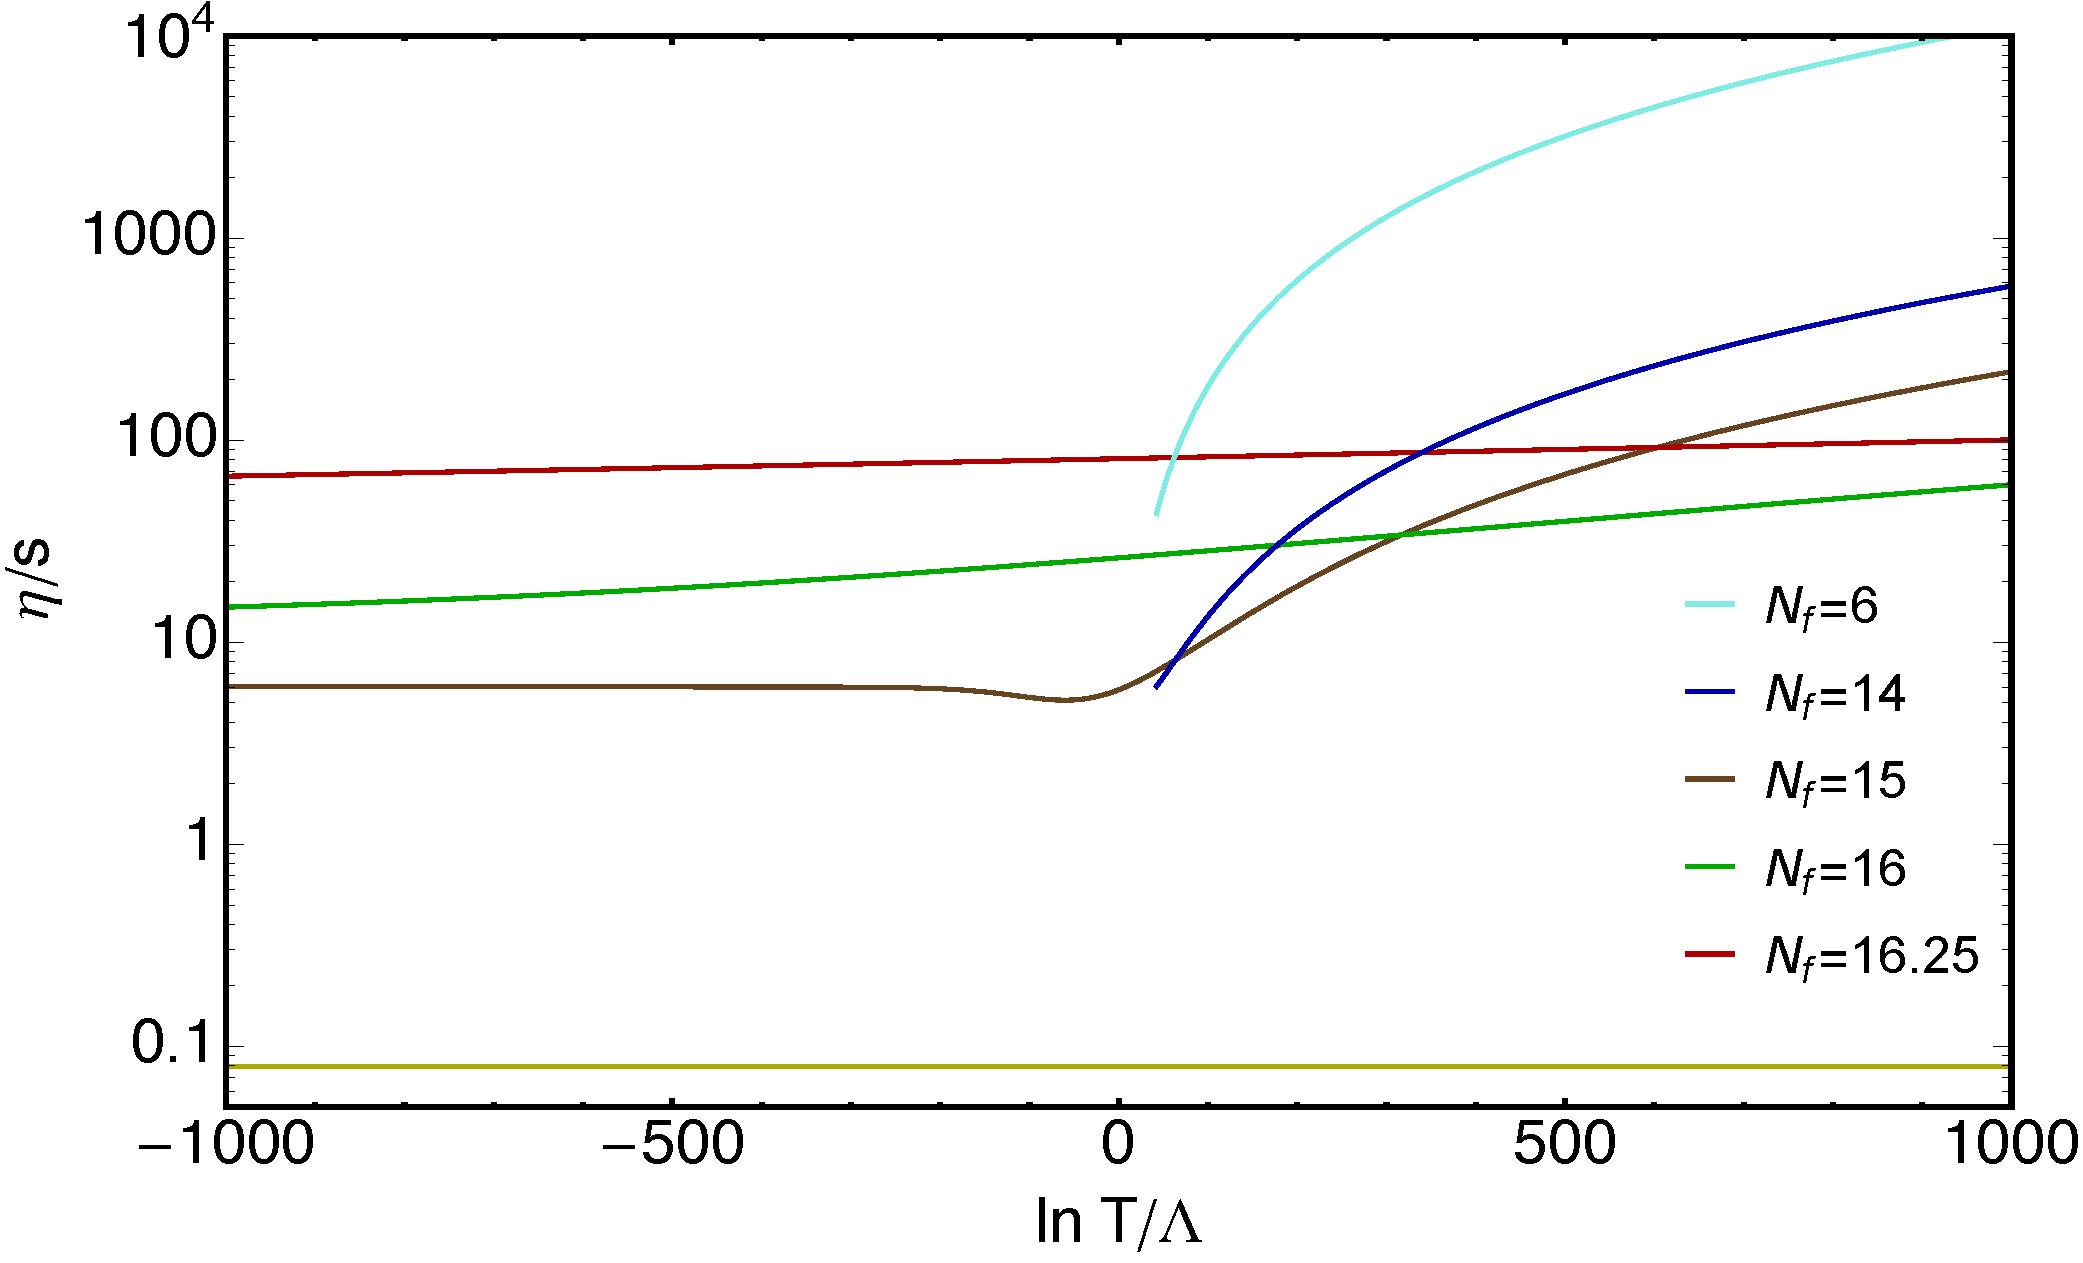
\includegraphics[width=0.68\textwidth]{pics/Temperature-etaovers-n3}
\end{center}
\caption{Upper panel: ${\eta}/{s}$ evaluated at the IR fixed point, as a function of the number of flavours, for fermions in 
the fundamental representation and $N = 3$ colours. Lower panel:  ${\eta}/{s}$ as function of the temperature over the 
RG scale $\Lambda$  for different values of $N_f$ in the conformal window and one outside corresponding to $N_f = 6$, for $N=3$ colours. Although $N_f = 14$ still displays a potential IR fixed point, the IR dynamics  of ${\eta}/{s}$ cannot be accessed perturbatively.  
The horizontal line at the bottom is the conjectured AdS/CFT bound. This picture has already been published in \cite{Toniato:2016twr}.} 
\label{etas_Nf}
\end{figure}

  
We repeat the above analysis for the fermion number diffusion coefficient. In the upper panel of figure \ref{D_Nf}, we plot the value of the dimensionless quantity $(T D)^{IR}$ as a function of $N_f$, for fermions in the fundamental representation and $N=3$. We linearly interpolate the values given in table \ref{AB} in order to express $B$ as a continuous function of $N_f$.
As for the case of the shear viscosity-to-entropy density ratio, we observe that $(TD)^{IR}$ diverges as the number of flavours approaches the asymptotic freedom boundary, corresponding to $g^* \to 0$. In the lower panel of figure \ref{D_Nf}, we plot $T D$ as a function of the temperature for different values of $N_f$ in the perturbative conformal window and for $N_f=6$. 

\begin{figure}[b!]
\begin{center}
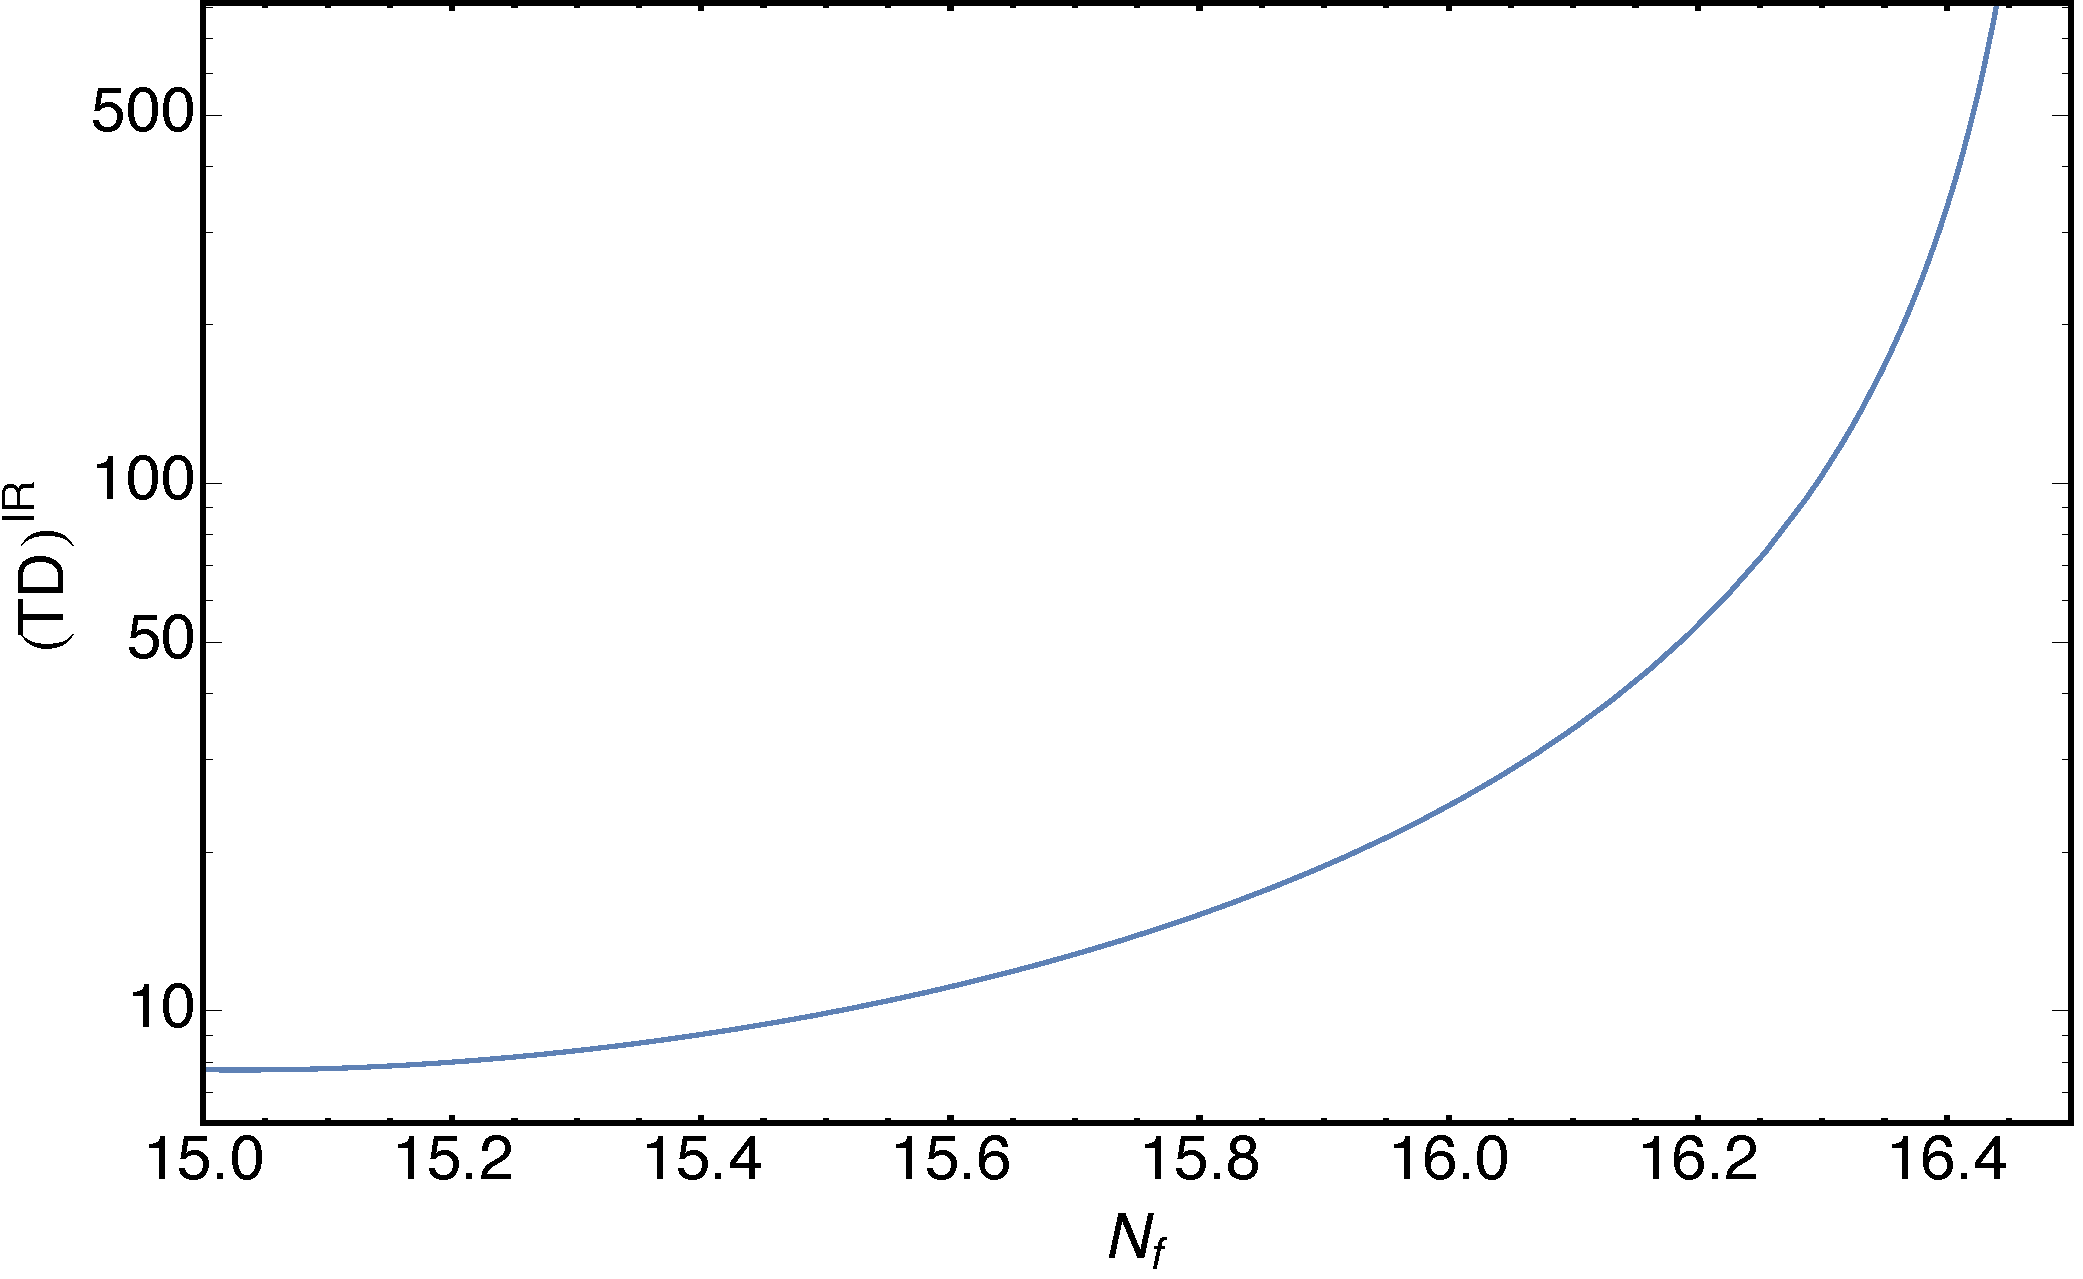
\includegraphics[width=0.665\textwidth]{pics/TDaN3} \\
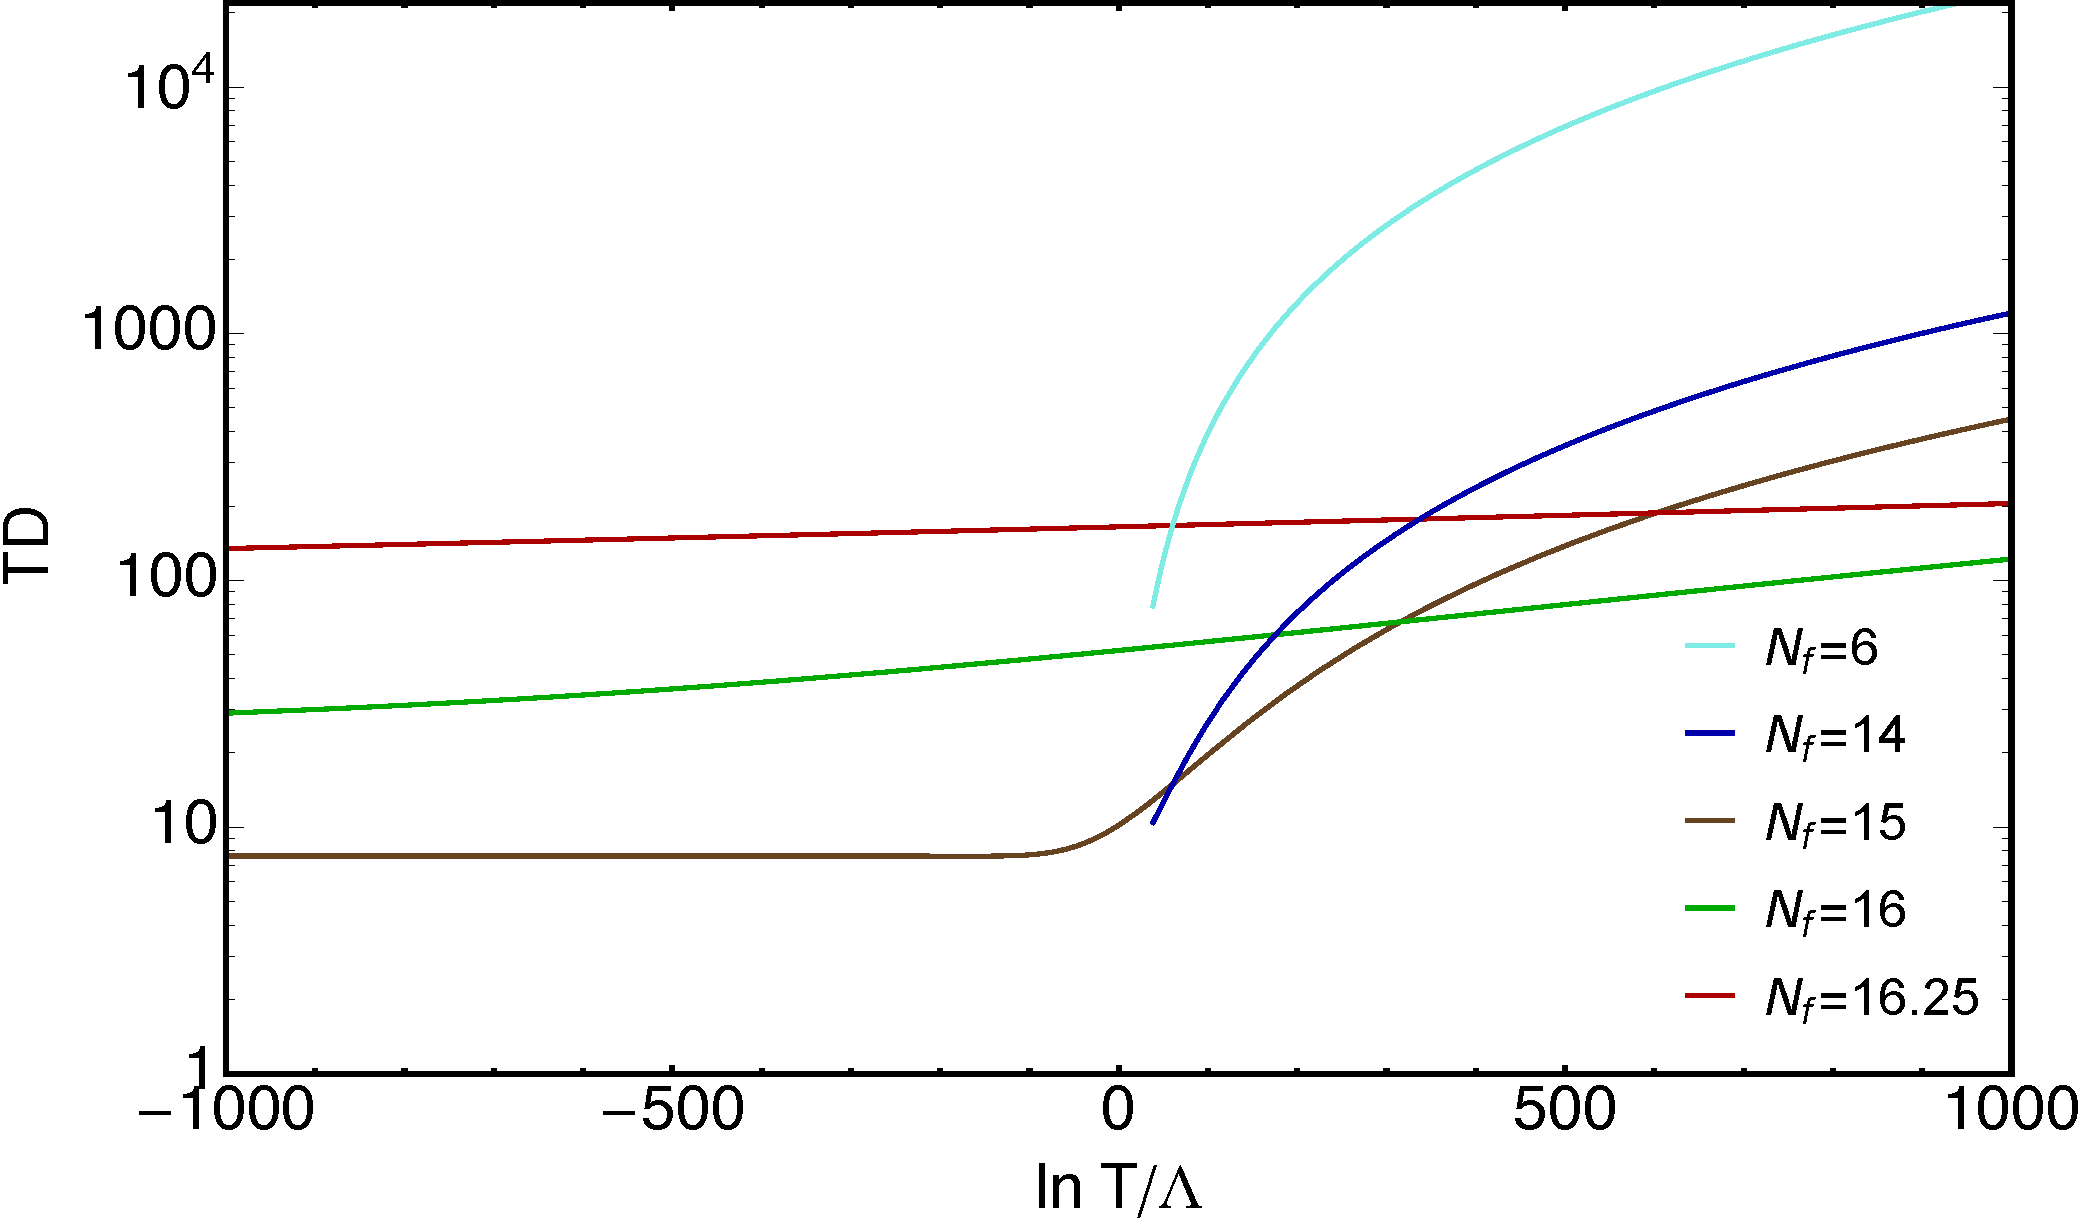
\includegraphics[width=0.7\textwidth]{pics/Temperature-TDaN3}
\end{center}
\caption{Upper panel: $(T D)^{IR}$ as a function of the number of flavours, for fermions in the fundamental representation and $N=3$. Lower panel: $T D$ as a function of the temperature, for different values of $N_f$ and $N=3$. This picture has already been published in \cite{Toniato:2016twr}.}
\label{D_Nf}
\end{figure}

One comment has to be made about the applicability of the next-to-leading-log approximation for transport coefficients in the conformal window. The presence of a perturbative IR fixed point allows us to apply the next-to-leading-log results in the whole energy range, from the UV (high temperature), where the theory is asymptotically free, down to the IR (low temperature). However, particular care has to be taken to decide whether the values obtained in the deep IR can be trusted. We chose to illustrate the results for the case of three colours and for different values of the number of flavours within the perturbative conformal window. $N_f=15$ is the last value at which we can observe the expected behaviour of the transport coefficients as functions of the temperature, i.e., to run from a divergent value in the UV down to a constant finite value in the IR. For $N_f=14$, the next-to-leading-log expression of the transport coefficients does not stabilise at a finite value in the IR, but instead diverges at low energies, showing that the next-to-leading-log approximation cannot be trusted even qualitatively. In fact, following \cite{Arnold:2003zc}, one can argue that the next-to-leading-log result is very close to the full-leading-order result (and therefore trustable) as long as $m_D/T \leq 1$.  This requirement is satisfied in our analysis provided $N_f \geq 16.25$, thus further limiting the window of applicability of the perturbative results.  The values of $m_D/T$ at the IR fixed point for $N=3$ and the values of $N_f$ within the conformal window considered in this study are reported in table \ref{mDTconstraint}.



   \begin{table}
\begin{center}
        \begin{tabular}{c||c }
    $N_f$ & $ \quad (m_D/T)^{IR}$ \\
    \hline \hline
        $14$ &$\quad 3.41$   \\
        $15$ & $\quad 2.51$ \\
        $16$ & $\quad 1.38$  \\
    $16.25$ & $\quad 0.97$ \\
    \end{tabular}
     \end{center}
\caption{Values of the ratio $m_D/T$ evaluated at the IR fixed point for $N=3$ and different values of $N_f$ in the 
conformal window. It can be observed that the constraint $m_D/T \leq 1$ is respected only in the case $N_f=16.25$.}
\label{mDTconstraint}
    \end{table}

To conclude, we summarise the salient points of our analysis. We determined the shear viscosity-to-entropy density ratio and the fermion number diffusion coefficient (multiplied by the temperature) within the perturbative regime of the conformal window. This provides a theoretically relevant example in which the perturbative estimate of the transport coefficients can be used along the entire RG flow from the UV to the IR without losing validity. We determined the range of applicability of those results within the conformal window of QCD-like theories. In the case $N=3$, we found out that already at $N_f=14$ the next-to-leading-log results cannot be trusted even qualitatively. The ratio $\eta/s$ at the IR fixed point drops significantly when going from 16.25 to 15 flavours showing that a modest change in the number of flavours dramatically affects the dynamics of the theory encoded in the transport coefficients. Higher-order corrections are needed to reach lower values of $N_f$ within the conformal window for the transport coefficients. In contrast, at zero temperature one observes that perturbation theory allows to go quite low in the number of flavours within the conformal window~\cite{Pica:2010mt,Pica:2010xq,Ryttov:2010iz,Ryttov:2016ner}. Although unproven, it is reasonable to expect that the minimum of $\eta/s$ as function of temperature in QCD lies below the lowest value of $\eta/s$ obtained at the bottom of the conformal window, and therefore lower than the one obtained near 15 flavours. 



%%%%%%%%%%%%%%%%%%%%%%%%%%%%%%%%%%%%%%%%%%%%%%%%%%%%%%
